\documentclass[preprint]{aastex} %double-column, single-spaced document:
%\documentclass[iop,floatfix]{emulateapj} 

\usepackage{hyperref}
%\usepackage{graphicx}
%\usepackage{apjfonts}
\usepackage{enumerate}
\usepackage{amsmath,amssymb}
\usepackage{geometry}
\usepackage{bm}
\usepackage[usenames,dvipsnames,svgnames,table]{xcolor}

\newcommand{\prob}{{\rm prob}}
\newcommand{\qN}{\{q_i\}_{i=1}^N}
\newcommand{\qM}{\{q_{im}\}_{i=1,m=0}^{N,M}}
\newcommand{\yN}{\{y_i\}_{i=1}^N}
\newcommand{\vt}{\vec{\theta}}
\newcommand{\vg}{\vt_{\star, {\rm grid}}}
\newcommand{\vpp}{\vt_{\star, {\rm post}}}
\newcommand{\vstar}{\vt_{\star}}
\newcommand{\vN}{\vt_{\rm N}}
\newcommand{\vc}{\vec{c}}
\newcommand{\fM}{ {\bm M}}
\newcommand{\fMi}{M_i}
\newcommand{\fD}{ {\bm D}}
\newcommand{\fDi}{D_i}
\newcommand{\dd}{\,{\rm d}}
\newcommand{\trans}{\mathsf{T}}
\newcommand{\Z}{[{\rm Fe}/{\rm H}]}
\newcommand{\A}{[\alpha/{\rm Fe}]}

\newcommand{\hcom}[1]{ \textcolor{Blue}{#1}}


%\slugcomment{}
%\shorttitle{}
%\shortauthors{}

\begin{document}

\title{Methods for the spectroscopic inference of fundamental stellar parameters, continued.}
\author{\today{}\\
\medskip
Ian~Czekala\altaffilmark{1} et al.
%Author2\altaffilmark{2},
}

\altaffiltext{1}{Harvard-Smithsonian Center for Astrophysics, 60 Garden Street MS 10, Cambridge, MA 02138}
%\altaffiltext{2}{Institution 2}
\email{iczekala@cfa.harvard.edu}

\section{Correlated noise}
\begin{itemize}
  \item \hcom{systematic errors don't necessarily invalidate chi-squared if they can be treated as a noise with a non-trivial covariance matrix; they just make chi-squared not an independent sum of residuals weighted by inverse variances but because a dot-product through a non-trivial inverse covariance tensor.}
  \item \hcom{"more drastic than adding in noise" -- what about "adding in highly covariant and correlated noise"? That takes no more equipment (everything is still Gaussian), but can handle far worse situations.}
  \item \hcom{Where you mention $\chi^2_Q$, you are treating the pixels as independent. But they aren't if there is model mismatch. That is, there are correlations among the residuals.}
\end{itemize}


Thank you for pointing this out. It spurred a bit of math on my part and now I've arrived at an interesting toy model that I would consider a nice proof-of-concept, although it has some major scaling problems. Maybe you could point to some good matrices routines.

Describe the $\chi^2$ for a non-trivial covariance matrix.

Describe how I determined the covariance function for a Gaussian. 

Show a plot of how using this covariance function one could generate noise that follows any range of values (a la ipython notebook).

Show the Bayesian model that uses the covariance function parameters, sparse matrices, and $\chi^2$. Show how it is able to correctly identify the parameters $b$, $m$, and the proper Gaussian noise values.

Ask about how to speed up this computation, or at least make some approximations. Note how similar it is to the ``add a line'' approach, though much more expensive. How to efficiently store matrix inversions? Is it necessary to actually compute the inverse?

Point out that different covariance functions could be useful for different spectral problems, such as M dwarf continuum (show reference, or lifted plot).

\begin{figure}[!htb]
\begin{center}
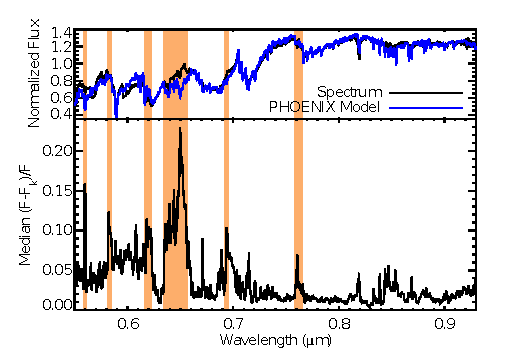
\includegraphics{mann}
\caption{From \citet{mga13}}
\label{fig:mann}
\end{center}
\end{figure}

good on the stuff about there being important information where the models and data disagree.

\hcom{in your four classes of line behavior, there is none which is dominated by continuum issues? Or is there? That is, continuum fitting can cause problems, no?}
I would think that yes, there should be areas where continuum fitting can be a problem. However, in the stars I'm looking at (over the narrow echelle range), the Chebyshev formalism essentially assumes that any continuum mis-match is actually a flux-calibration (instrumental) issue, and accounts for it. This means that if we were fitting hotter stars with few lines, any information contained in the continuum shape would be lost. However, this approach does prevent against introducing bad features \emph{into} the continuum.

Depending on the size of the continuum problem, yes, this may also be a problem. I didn't include it in the error classification because I didn't think it was as dire a problem as the others, but when it comes to M spectra, this may actually be a problem.

\hcom{trigger went off with "making these regions useless for determining...". Useless?}
I shouldn't have been so hasty!

\hcom{Section 5: You might even be able to learn changes to the models. This is the holy grail.}
I see where this is going. In the original approach I could plot the sparsity matrix, and the areas of larger variance/off-diagonal terms would pin-point where the model and data diverge. Also, the form of the covariance function.

\section{Downsampling}

\hcom{section 2: why "linearly interpolate"? It would be good to see more specificity here; there are lots of ways to do this smooth and downsample slightly wrong.}

For the linear interpolation from the grid, basically it is because I wanted implement my lnprob easily and to be memory efficient. It would be better to use a more sophisticated interpolator. For example, \citet{hwd+13} use a spline interpolator (I think), where they pre-compute and store the derivatives of the spectra. This is currently low priority because we expect the actual error to be due to these systematic errors in the model.

I went through a few of the wrong approaches. Allow me to elaborate on the current method.
Keep Fourier in touch. Spectra from the PHOENIX grid are given in units of flux density. We flux calibrate our spectra, so that they are also in flux density.

\section{Chebyshev}
\hcom{Can you really marginalize analytically over the Chebyshev polynomials? And doesn't that make a huge, correlated uncertainty tensor? And what priors do you use?}
I'm uncertain what you mean about the huge, correlated uncertainty tensor. Which parameters are in this tensor? 

\hcom{In re +/- 0.01 dex: You have tons of pixels so of course you get amazing constraints! It would be surprising if you didn't. But do you get such amazing constraints if you marginalize analytically over thousands of Chebyshevs?}
Show plot of run output, things still work fine, and in fact you get the same answer sampled vs. marginalized?

\hcom{When you do the drop and interpolate over testing, can you build an empirical interpolation error model and then use it?}
I am planning on building a model, but it has been lower priority at the moment. 






\bibliography{disks,bayesian,master}
\bibliographystyle{hapj}
\end{document}
